\section{Introduction}
\label{ch:Introduction}

\begin{figure*}[hbt!]
    \centering
    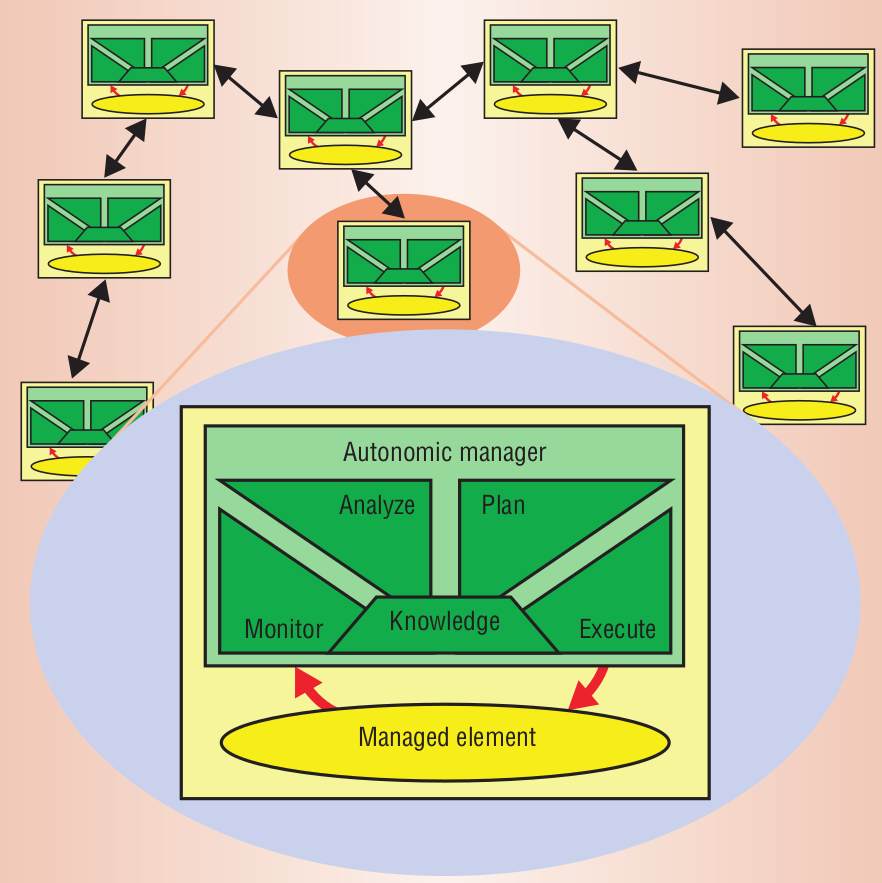
\includegraphics[width=0.6\textwidth]{images/MAPEK.png}
    \caption{The \acrshort{mapek} (Monitor-Analyze-Plan-Execute with Knowledge) feedback loop by Kephart and Chess, 2003 \cite*{VisionOfAutonomicComputing}}
    \label{fig:MAPEK}
\end{figure*}

The complexity of modern software systems is constantly growing.
Most of this growth in complexity stems from the
"need to integrate several heterogeneous environments into corporate-wide computing systems,
and to extend that beyond company boundaries into the Internet" (Kephart and Chess, 2003 \cite*{VisionOfAutonomicComputing}).
This has reached a state where the
"complexity appears to be approaching the limits of human capability" (Kephart and Chess, 2003 \cite*{VisionOfAutonomicComputing}).
In combination with the uncertainty about a software systems future operations and environment,
that the developers of such complex systems face, it becomes uneconomical to purely operate such a system by human operators.

\noindent From this the need for software systems which can autonomously manage themselves arises.
In order to achieve this task of autonomous self-management, the system has to be able to:
\begin{itemize}[nosep]
    \item detect faults and changes in its environment,
    \item analyze them,
    \item decide how to react to them
    \item and make changes to itself.
\end{itemize}

\newpage
\noindent To model these abilities Kephart and Chess developed
the \acrfull{mapek} feedback loop \cite*{VisionOfAutonomicComputing} shown in Figure \ref{fig:MAPEK}.

\noindent First the system has to \textit{monitor} itself and its environment.
The data, gathered by the monitoring step, has to be \textit{analyzed} to detect changes and faults.
If the analyzing step detects, that an adaptation is necessary,
the system has to \textit{plan} how to perform the necessary changes.
After the changes have been planned, they need to be \textit{executed}.
All of this happens with \textit{knowledge} of the environment and the system.

\noindent Software systems that can autonomously manage themselves are called \acrfull{sas}[s]
because of their ability to adapt themselves.

\noindent To better understand \acrshort{sas}, let us take a look at a commonly used example.
Imaging you are the system administrator of a large scale online store.
This store has four parameters: site traffic, number of purchases, number of active server instances and the number of served advertisements.
During your day to day operations you encounter a common type of task:
Update some system parameter X based on some metric Y.
To make your job easier, you decide to use a \acrshort{sas} for these tasks
and come up with the following generalized adaptation rule:
If metric Y crosses threshold Z, update the system parameter X.

\noindent In this case the usage of a \acrshort{sas} was beneficial because it could easily
automate a general set of tasks.
A human operator might have been able to perform these tasks on his own,
if the number of system parameters was sufficiently small.
But the \acrshort{sas} is better at handling large numbers of system parameters.


\noindent While \acrshort{sas} are better at handling more complex systems,
human operators are better at handling uncertainty.
This has two reasons. 
Firstly, the adaptation rules and policies used by \acrshort{sas} are statically created at design time.
Secondly, \acrshort{sas} can adapt the software that they are managing but they can not change their adaptation process.
Over time this leads to an increasing divergence between the expected results of adaptations and the actual results,
when the environment changes in ways that were not predicted by developers during the design time of the system.

\noindent This can be illustrated by the previous example.
Imagine that the \acrshort{sas} has been in operation for some and you collected data on the systems performance.
You notice that the \acrshort{sas} changes some system parameters too aggressively,
because it performs an adaptation as soon as a metrics threshold has been violated.
As a human operator you would have waited some time to see how the metric develops before performing an adaptation
which would result in a smoother operation.
The \acrshort{sas} can not handle this type of uncertainty and only reacted to the current state of its environment.

\noindent Optimizations are necessary to improve the performance and effectiveness of \acrshort{sas} in situations like these.
There are already many approaches on how to optimize \acrshort{sas}.
Some of them focus on updating adaptation rules and policies during the systems runtime.
Others dynamically change at which level of the system adaptations are performed.
Generally most optimizations target static components of \acrshort{sas}.
These components can be improved by making them more dynamic, 
which is often achieved by applying modern learning methods.

\noindent The previous example could benefit from such optimizations by dynamically updating adaptation rules
to better reflect the systems changing environment.

\noindent While there are already many \acrfull{oa}[es] for \acrshort{sas},
there is no classification for them.
Because of this, the existing \acrshort{oa} can not be easily compared
and it is difficult to identify areas which require further research.
This paper aims to provide such a classification for \acrlong{oa}[es] for \acrlong{sas}[s].

\noindent To derive a classification for \acrshort{oa} for \acrshort{sas},
chapter \ref{ch:SASClassification} will first explain how \acrshort{sas} are classified
using three different approaches.
Based on these approaches, a classification for \acrshort{oa} for \acrshort{sas} will be derived
and proposed in chapter \ref{ch:Proposal}.
In chapter \ref{ch:Existing} the proposed classification will be applied to some existing \acrshort{oa}.
Lastly, chapter \ref{ch:Conclusion} will finish with a conclusion and recommendations for future research directions.
